\chapter{Valentine}

We may easily conceive where Morrel’s appointment was. On leaving Monte
Cristo he walked slowly towards Villefort’s; we say slowly, for Morrel
had more than half an hour to spare to go five hundred steps, but he
had hastened to take leave of Monte Cristo because he wished to be
alone with his thoughts. He knew his time well—the hour when Valentine
was giving Noirtier his breakfast, and was sure not to be disturbed in
the performance of this pious duty. Noirtier and Valentine had given
him leave to go twice a week, and he was now availing himself of that
permission.

He arrived; Valentine was expecting him. Uneasy and almost crazed, she
seized his hand and led him to her grandfather. This uneasiness,
amounting almost to frenzy, arose from the report Morcerf’s adventure
had made in the world, for the affair at the Opera was generally known.
No one at Villefort’s doubted that a duel would ensue from it.
Valentine, with her woman’s instinct, guessed that Morrel would be
Monte Cristo’s second, and from the young man’s well-known courage and
his great affection for the count, she feared that he would not content
himself with the passive part assigned to him. We may easily understand
how eagerly the particulars were asked for, given, and received; and
Morrel could read an indescribable joy in the eyes of his beloved, when
she knew that the termination of this affair was as happy as it was
unexpected.

“Now,” said Valentine, motioning to Morrel to sit down near her
grandfather, while she took her seat on his footstool,—“now let us talk
about our own affairs. You know, Maximilian, grandpapa once thought of
leaving this house, and taking an apartment away from M. de
Villefort’s.”

“Yes,” said Maximilian, “I recollect the project, of which I highly
approved.”

“Well,” said Valentine, “you may approve again, for grandpapa is again
thinking of it.”

“Bravo,” said Maximilian.

\begin{figure}[ht]
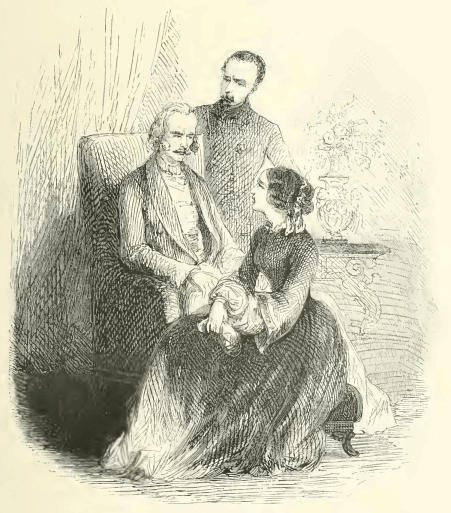
\includegraphics[width=\textwidth]{40272m.jpg}
\end{figure}

“And do you know,” said Valentine, “what reason grandpapa gives for
leaving this house.” Noirtier looked at Valentine to impose silence,
but she did not notice him; her looks, her eyes, her smile, were all
for Morrel.

“Oh, whatever may be M. Noirtier’s reason,” answered Morrel, “I can
readily believe it to be a good one.”

“An excellent one,” said Valentine. “He pretends the air of the
Faubourg Saint-Honoré is not good for me.”

“Indeed?” said Morrel; “in that M. Noirtier may be right; you have not
seemed to be well for the last fortnight.”

“Not very,” said Valentine. “And grandpapa has become my physician, and
I have the greatest confidence in him, because he knows everything.”

“Do you then really suffer?” asked Morrel quickly.

“Oh, it must not be called suffering; I feel a general uneasiness, that
is all. I have lost my appetite, and my stomach feels as if it were
struggling to get accustomed to something.” Noirtier did not lose a
word of what Valentine said.

“And what treatment do you adopt for this singular complaint?”

“A very simple one,” said Valentine. “I swallow every morning a
spoonful of the mixture prepared for my grandfather. When I say one
spoonful, I began by one—now I take four. Grandpapa says it is a
panacea.” Valentine smiled, but it was evident that she suffered.

Maximilian, in his devotedness, gazed silently at her. She was very
beautiful, but her usual pallor had increased; her eyes were more
brilliant than ever, and her hands, which were generally white like
mother-of-pearl, now more resembled wax, to which time was adding a
yellowish hue.

From Valentine the young man looked towards Noirtier. The latter
watched with strange and deep interest the young girl, absorbed by her
affection, and he also, like Morrel, followed those traces of inward
suffering which was so little perceptible to a common observer that
they escaped the notice of everyone but the grandfather and the lover.

“But,” said Morrel, “I thought this mixture, of which you now take four
spoonfuls, was prepared for M. Noirtier?”

“I know it is very bitter,” said Valentine; “so bitter, that all I
drink afterwards appears to have the same taste.” Noirtier looked
inquiringly at his granddaughter. “Yes, grandpapa,” said Valentine; “it
is so. Just now, before I came down to you, I drank a glass of sugared
water; I left half, because it seemed so bitter.” Noirtier turned pale,
and made a sign that he wished to speak.

Valentine rose to fetch the dictionary. Noirtier watched her with
evident anguish. In fact, the blood was rushing to the young girl’s
head already, her cheeks were becoming red.

“Oh,” cried she, without losing any of her cheerfulness, “this is
singular! I can’t see! Did the sun shine in my eyes?” And she leaned
against the window.

“The sun is not shining,” said Morrel, more alarmed by Noirtier’s
expression than by Valentine’s indisposition. He ran towards her. The
young girl smiled.

“Cheer up,” said she to Noirtier. “Do not be alarmed, Maximilian; it is
nothing, and has already passed away. But listen! Do I not hear a
carriage in the courtyard?” She opened Noirtier’s door, ran to a window
in the passage, and returned hastily. “Yes,” said she, “it is Madame
Danglars and her daughter, who have come to call on us. Good-bye;—I
must run away, for they would send here for me, or, rather, farewell
till I see you again. Stay with grandpapa, Maximilian; I promise you
not to persuade them to stay.”

\begin{figure}[ht]
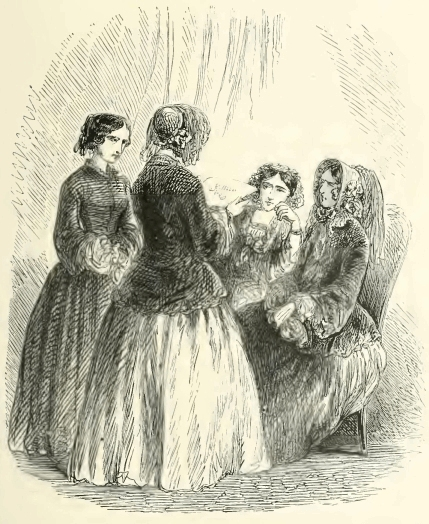
\includegraphics[width=\textwidth]{40274m.jpg}
\end{figure}

Morrel watched her as she left the room; he heard her ascend the little
staircase which led both to Madame de Villefort’s apartments and to
hers. As soon as she was gone, Noirtier made a sign to Morrel to take
the dictionary. Morrel obeyed; guided by Valentine, he had learned how
to understand the old man quickly. Accustomed, however, as he was to
the work, he had to repeat most of the letters of the alphabet and to
find every word in the dictionary, so that it was ten minutes before
the thought of the old man was translated by these words,

“Fetch the glass of water and the decanter from Valentine’s room.”

Morrel rang immediately for the servant who had taken Barrois’s
situation, and in Noirtier’s name gave that order. The servant soon
returned. The decanter and the glass were completely empty. Noirtier
made a sign that he wished to speak.

“Why are the glass and decanter empty?” asked he; “Valentine said she
only drank half the glassful.”

The translation of this new question occupied another five minutes.

“I do not know,” said the servant, “but the housemaid is in
Mademoiselle Valentine’s room: perhaps she has emptied them.”

“Ask her,” said Morrel, translating Noirtier’s thought this time by his
look. The servant went out, but returned almost immediately.
“Mademoiselle Valentine passed through the room to go to Madame de
Villefort’s,” said he; “and in passing, as she was thirsty, she drank
what remained in the glass; as for the decanter, Master Edward had
emptied that to make a pond for his ducks.”

Noirtier raised his eyes to heaven, as a gambler does who stakes his
all on one stroke. From that moment the old man’s eyes were fixed on
the door, and did not quit it.

It was indeed Madame Danglars and her daughter whom Valentine had seen;
they had been ushered into Madame de Villefort’s room, who had said she
would receive them there. That is why Valentine passed through her
room, which was on a level with Valentine’s, and only separated from it
by Edward’s. The two ladies entered the drawing-room with that sort of
official stiffness which preludes a formal communication. Among worldly
people manner is contagious. Madame de Villefort received them with
equal solemnity. Valentine entered at this moment, and the formalities
were resumed.

“My dear friend,” said the baroness, while the two young people were
shaking hands, “I and Eugénie are come to be the first to announce to
you the approaching marriage of my daughter with Prince Cavalcanti.”
Danglars kept up the title of prince. The popular banker found that it
answered better than count.

“Allow me to present you my sincere congratulations,” replied Madame de
Villefort. “Prince Cavalcanti appears to be a young man of rare
qualities.”

\begin{figure}[ht]
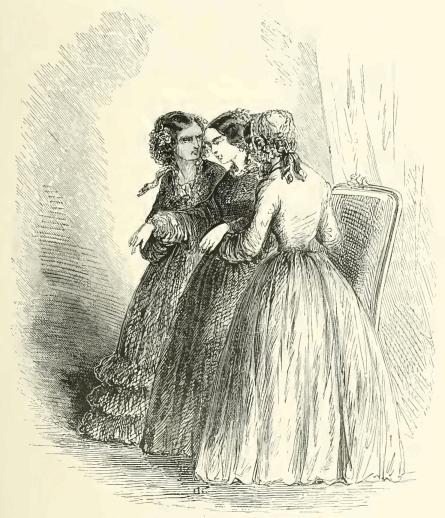
\includegraphics[width=\textwidth]{40276m.jpg}
\end{figure}

“Listen,” said the baroness, smiling; “speaking to you as a friend I
can say that the prince does not yet appear all he will be. He has
about him a little of that foreign manner by which French persons
recognize, at first sight, the Italian or German nobleman. Besides, he
gives evidence of great kindness of disposition, much keenness of wit,
and as to suitability, M. Danglars assures me that his fortune is
majestic—that is his word.”

“And then,” said Eugénie, while turning over the leaves of Madame de
Villefort’s album, “add that you have taken a great fancy to the young
man.”

“And,” said Madame de Villefort, “I need not ask you if you share that
fancy.”

“I?” replied Eugénie with her usual candor. “Oh, not the least in the
world, madame! My wish was not to confine myself to domestic cares, or
the caprices of any man, but to be an artist, and consequently free in
heart, in person, and in thought.”

Eugénie pronounced these words with so firm a tone that the color
mounted to Valentine’s cheeks. The timid girl could not understand that
vigorous nature which appeared to have none of the timidities of woman.

“At any rate,” said she, “since I am to be married whether I will or
not, I ought to be thankful to Providence for having released me from
my engagement with M. Albert de Morcerf, or I should this day have been
the wife of a dishonored man.”

“It is true,” said the baroness, with that strange simplicity sometimes
met with among fashionable ladies, and of which plebeian intercourse
can never entirely deprive them,—“it is very true that had not the
Morcerfs hesitated, my daughter would have married Monsieur Albert. The
general depended much on it; he even came to force M. Danglars. We have
had a narrow escape.”

“But,” said Valentine, timidly, “does all the father’s shame revert
upon the son? Monsieur Albert appears to me quite innocent of the
treason charged against the general.”

“Excuse me,” said the implacable young girl, “Monsieur Albert claims
and well deserves his share. It appears that after having challenged M.
de Monte Cristo at the Opera yesterday, he apologized on the ground
today.”

“Impossible,” said Madame de Villefort.

“Ah, my dear friend,” said Madame Danglars, with the same simplicity we
before noticed, “it is a fact. I heard it from M. Debray, who was
present at the explanation.”

Valentine also knew the truth, but she did not answer. A single word
had reminded her that Morrel was expecting her in M. Noirtier’s room.
Deeply engaged with a sort of inward contemplation, Valentine had
ceased for a moment to join in the conversation. She would, indeed,
have found it impossible to repeat what had been said the last few
minutes, when suddenly Madame Danglars’ hand, pressed on her arm,
aroused her from her lethargy.

“What is it?” said she, starting at Madame Danglars’ touch as she would
have done from an electric shock.

“It is, my dear Valentine,” said the baroness, “that you are,
doubtless, suffering.”

\begin{figure}[ht]
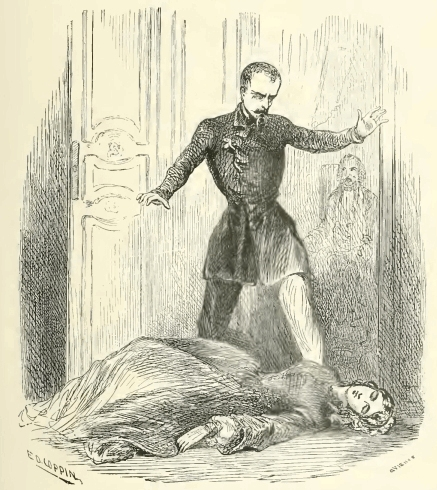
\includegraphics[width=\textwidth]{40280m.jpg}
\end{figure}

“I?” said the young girl, passing her hand across her burning forehead.

“Yes, look at yourself in that glass; you have turned pale and then red
successively, three or four times in one minute.”

“Indeed,” cried Eugénie, “you are very pale!”

“Oh, do not be alarmed; I have been so for many days.” Artless as she
was, the young girl knew that this was an opportunity to leave, and
besides, Madame de Villefort came to her assistance.

“Retire, Valentine,” said she; “you are really suffering, and these
ladies will excuse you; drink a glass of pure water, it will restore
you.”

Valentine kissed Eugénie, bowed to Madame Danglars, who had already
risen to take her leave, and went out.

“That poor child,” said Madame de Villefort when Valentine was gone,
“she makes me very uneasy, and I should not be astonished if she had
some serious illness.”

Meanwhile, Valentine, in a sort of excitement which she could not quite
understand, had crossed Edward’s room without noticing some trick of
the child, and through her own had reached the little staircase.

She was within three steps of the bottom; she already heard Morrel’s
voice, when suddenly a cloud passed over her eyes, her stiffened foot
missed the step, her hands had no power to hold the baluster, and
falling against the wall she lost her balance wholly and toppled to the
floor. Morrel bounded to the door, opened it, and found Valentine
stretched out at the bottom of the stairs. Quick as a flash, he raised
her in his arms and placed her in a chair. Valentine opened her eyes.

“Oh, what a clumsy thing I am,” said she with feverish volubility; “I
don’t know my way. I forgot there were three more steps before the
landing.”

“You have hurt yourself, perhaps,” said Morrel. “What can I do for you,
Valentine?”

Valentine looked around her; she saw the deepest terror depicted in
Noirtier’s eyes.

“Don’t worry, dear grandpapa,” said she, endeavoring to smile; “it is
nothing—it is nothing; I was giddy, that is all.”

“Another attack of giddiness,” said Morrel, clasping his hands. “Oh,
attend to it, Valentine, I entreat you.”

“But no,” said Valentine,—“no, I tell you it is all past, and it was
nothing. Now, let me tell you some news; Eugénie is to be married in a
week, and in three days there is to be a grand feast, a betrothal
festival. We are all invited, my father, Madame de Villefort, and I—at
least, I understood it so.”

“When will it be our turn to think of these things? Oh, Valentine, you
who have so much influence over your grandpapa, try to make him
answer—Soon.”

“And do you,” said Valentine, “depend on me to stimulate the tardiness
and arouse the memory of grandpapa?”

“Yes,” cried Morrel, “make haste. So long as you are not mine,
Valentine, I shall always think I may lose you.”

“Oh,” replied Valentine with a convulsive movement, “oh, indeed,
Maximilian, you are too timid for an officer, for a soldier who, they
say, never knows fear. Ha, ha, ha!”

She burst into a forced and melancholy laugh, her arms stiffened and
twisted, her head fell back on her chair, and she remained motionless.
The cry of terror which was stopped on Noirtier’s lips, seemed to start
from his eyes. Morrel understood it; he knew he must call assistance.
The young man rang the bell violently; the housemaid who had been in
Mademoiselle Valentine’s room, and the servant who had replaced
Barrois, ran in at the same moment. Valentine was so pale, so cold, so
inanimate that without listening to what was said to them they were
seized with the fear which pervaded that house, and they flew into the
passage crying for help. Madame Danglars and Eugénie were going out at
that moment; they heard the cause of the disturbance.

“I told you so!” exclaimed Madame de Villefort. “Poor child!”

\begin{figure}[ht]
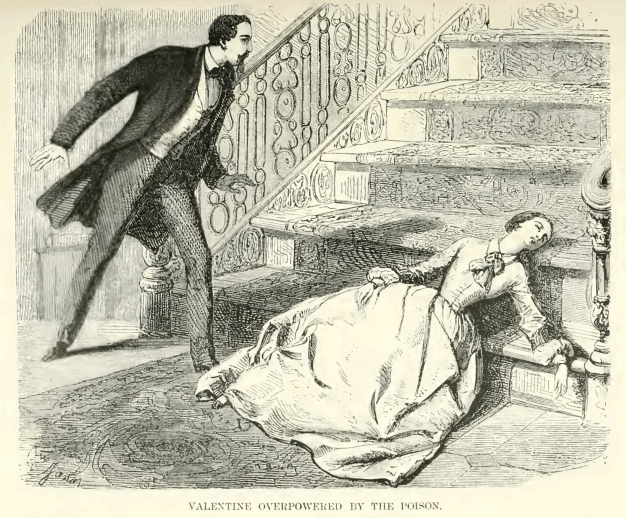
\includegraphics[width=\textwidth]{40278m.jpg}
\end{figure}
